%!TEX program = pdflatex
\documentclass[10pt]{beamer}

\usepackage{tikz}
\usepackage{pgfplots}
\pgfplotsset{compat=1.10}

\usetheme{Warsaw}
\usefonttheme{serif}
\usepackage{mathpazo}
 % 定义一个整体的缩放比例参数,否则会导致图形缩放了,而文本没有相等比例的缩放
\tikzset{global scale/.style={
    scale=#1,
    every node/.style={scale=#1}
  }
}
 % 定义正态分布函数
\pgfmathdeclarefunction{gauss}{2}{%
  \pgfmathparse{1/(#2*sqrt(2*pi))*exp(-((x-#1)^2)/(2*#2^2))}%
}

 % 根据两个均值,求出正态分布上的点的值
\def\x{-0.5}
\def\fx{1/(1.3*sqrt(2*pi))*exp(-((\x+0.5)^2)/(2*1.3^2))}
\def\y{1}
\def\fy{1/(0.9*sqrt(2*pi))*exp(-((\y-1)^2)/(2*0.9^2))}

\begin{document}

\begin{frame}[t]\frametitle{Overlay}

\begin{center}
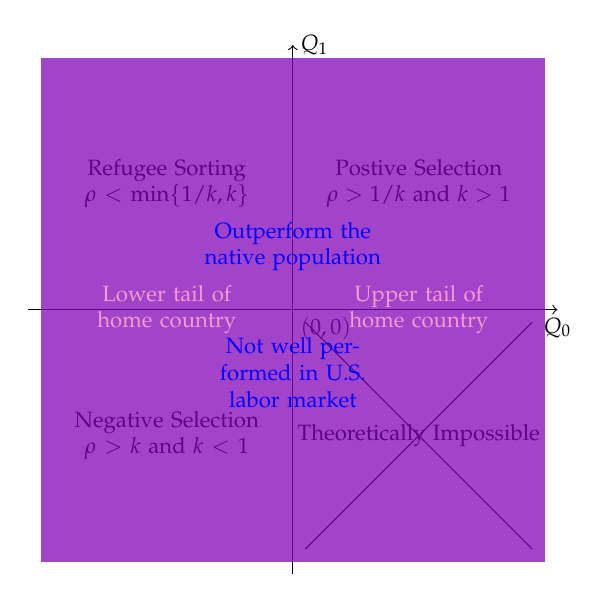
\begin{tikzpicture}[global scale=0.8]
 % 画出两个坐标轴,并标注为 Q0 和 Q1
\draw[->] (-4.2,0) -- (4.2,0) node[below]{$Q_{0}$};
\draw[->] (0,-4.2) -- (0,4.2) node[right]{$Q_{1}$};
\draw (0,0) node[anchor=north west]{$(0,0)$};
 % 填充第一象限
\visible<1->{
\fill[gray,opacity=0.2] (0,0) rectangle (4,4);
\draw (2,2) node[text width=3cm,align=center]{\alert{Postive Selection} $\rho > 1/k \mbox{ and } k > 1$};}
 % 填充第二象限
\visible<2->{
\fill[gray,opacity=0.2] (0,0) rectangle (-4,-4);
\draw (-2,-2) node[text width=3cm,align=center]{\alert{Negative Selection} $\rho > k \mbox{ and } k < 1$};}
 % 填充第三象限
\visible<3->{
\fill[gray,opacity=0.2] (0,0) rectangle (-4,4);
\draw (-2,2) node[text width=3cm,align=center]{\alert{Refugee Sorting} $\rho < \min\{1/k,k\}$}; }
 % 填充第四象限 + 两个直线
\visible<4->{
\fill[gray,opacity=0.2] (0,0) rectangle (4,-4);
\draw (0.2,-0.2) -- (3.8,-3.8);
\draw (3.8,-0.2) -- (0.2,-3.8);
\draw (2,-2) node[text width=5cm,align=center]{\alert{Theoretically Impossible} };}
 % 填充第一、第四象限
\visible<5-6>{
\fill[blue,opacity=0.5] (0,-4) rectangle (4,4);
\draw (2,0) node[text width=3cm,align=center]{\textcolor{white}{Upper tail of home country} };}
 % 填充第二、第三象限
\visible<6-6>{
\fill[blue,opacity=0.5] (0,-4) rectangle (-4,4);
\draw (-2,0) node[text width=3cm,align=center]{\textcolor{white}{Lower tail of home country} };}
 % 填充第一、第二象限
\visible<7-8>{
\fill[magenta,opacity=0.4] (-4,0) rectangle (4,4);
\draw (0,1) node[text width=3cm,align=center]{\textcolor{blue}{Outperform the native population} };}
 % 填充第三、第四象限
\visible<8-8>{
\fill[magenta,opacity=0.4] (-4,0) rectangle (4,-4);
\draw (0,-1) node[text width=3cm,align=center]{\textcolor{blue}{Not well performed  in U.S. labor market} };}
\end{tikzpicture}
\end{center}

\end{frame}


\begin{frame}[c]\frametitle{Normal Density}

\begin{center}
\begin{tikzpicture}[global scale = 0.85]
 % 画出坐标轴,不需要 x 和 y 的轴线,不标注
\begin{axis}[axis x line=none, axis y line = none,xtick=\empty,ytick=\empty,every axis plot post/.append style={domain=-5:5,samples=50,smooth}]
  \addplot[magenta] {gauss(1,0.9)}; % 添加正态分布曲线 1
  \addplot[blue] {gauss(-0.5,1.3)}; % 添加正态分布曲线 2
  \draw (axis cs:-5,0) -- (axis cs:5,0); % 添加一根直线,作为轴线的替代

  \draw[dashed] (axis cs:{\x},{\fx}) -- (axis cs:{\x},0) node[below]{$\mu_{0}+\pi$}; % 从正态分布 1 的顶端画一根垂线下来,交于 x 轴
  \draw[dashed] (axis cs:{\y},{\fy}) -- (axis cs:{\y},0) node[below]{$\mu_{1}$}; % 从正态分布 2 的顶端画一根垂线下来,交于 x 轴
  \node at (axis cs: -3, 0.3){$\sigma_{1} < \sigma_{0}$}; % 文本标注

  \only<2->{\addplot[blue] {gauss(-0.5,1.8)}; % 添加另外一根正态分布曲线
  \node at (axis cs: -3, 0.2){\textcolor{blue}{$\sigma_{0}^{\prime} > \sigma_{0}$}};}
\end{axis}
\end{tikzpicture}
\end{center}

\end{frame}

\end{document}
